\documentclass[a4paper]{article}
\usepackage[spanish]{babel}
\usepackage[utf8]{inputenc}
\usepackage{charter}   % tipografia
\usepackage{graphicx}
%\usepackage{makeidx}
\usepackage{paralist} %itemize inline

%\usepackage{float}
%\usepackage{amsmath, amsthm, amssymb}
%\usepackage{amsfonts}
%\usepackage{sectsty}
%\usepackage{charter}
%\usepackage{wrapfig}
%\usepackage{listings}
%\lstset{language=C}
\usepackage{bm} %bold math symbols


\usepackage{color} % para snipets de codigo coloreados
\usepackage{fancybox}  % para el sbox de los snipets de codigo

\definecolor{litegrey}{gray}{0.94}

% \newenvironment{sidebar}{%
% 	\begin{Sbox}\begin{minipage}{.85\textwidth}}%
% 	{\end{minipage}\end{Sbox}%
% 		\begin{center}\setlength{\fboxsep}{6pt}%
% 		\shadowbox{\TheSbox}\end{center}}
% \newenvironment{warning}{%
% 	\begin{Sbox}\begin{minipage}{.85\textwidth}\sffamily\lite\small\RaggedRight}%
% 	{\end{minipage}\end{Sbox}%
% 		\begin{center}\setlength{\fboxsep}{6pt}%
% 		\colorbox{litegrey}{\TheSbox}\end{center}}

\newenvironment{codesnippet}{%
	\begin{Sbox}\begin{minipage}{\textwidth}\sffamily\small}%
	{\end{minipage}\end{Sbox}%
		\begin{center}%
		\vspace{-0.4cm}\colorbox{litegrey}{\TheSbox}\end{center}\vspace{0.3cm}}



\usepackage{fancyhdr}
\pagestyle{fancy}

%\renewcommand{\chaptermark}[1]{\markboth{#1}{}}
\renewcommand{\sectionmark}[1]{\markright{\thesection\ - #1}}

\fancyhf{}

\fancyhead[LO]{Sección \rightmark} % \thesection\ 
\fancyfoot[LO]{\small{Cort\'es Lucas, Zimenspitz Ezequiel, Lamela Emanuel}}
\fancyfoot[RO]{\thepage}
\renewcommand{\headrulewidth}{0.5pt}
\renewcommand{\footrulewidth}{0.5pt}
\setlength{\hoffset}{-0.8in}
\setlength{\textwidth}{16cm}
%\setlength{\hoffset}{-1.1cm}
%\setlength{\textwidth}{16cm}
\setlength{\headsep}{0.5cm}
\setlength{\textheight}{25cm}
\setlength{\voffset}{-0.7in}
\setlength{\headwidth}{\textwidth}
\setlength{\headheight}{13.1pt}

\renewcommand{\baselinestretch}{1.1}  % line spacing


% \setcounter{secnumdepth}{2}
\usepackage{underscore}
\usepackage{caratula}
\usepackage{url}


% ******************************************************** %
%              TEMPLATE DE INFORME ORGA2 v0.1              %
% ******************************************************** %
% ******************************************************** %
%                                                          %
% ALGUNOS PAQUETES REQUERIDOS (EN UBUNTU):                 %
% ========================================
%                                                          %
% texlive-latex-base                                       %
% texlive-latex-recommended                                %
% texlive-fonts-recommended                                %
% texlive-latex-extra?                                     %
% texlive-lang-spanish (en ubuntu 13.10)                   %
% ******************************************************** %



\begin{document}

\thispagestyle{empty}
\materia{M\'etodos Num\'ericos}
\submateria{Primer Cuatrimestre de 2016}
\titulo{Trabajo Práctico I}
\subtitulo{(No) Todo Pasa}
\integrante{Cort\'es, Lucas}{302/13}{lucascortes@me.com}
\integrante{Lamela, Emanuel}{021/13}{emanuel93_13@hotmail.com}
\integrante{Zimenspitz, Ezequiel}{155/13}{ezeqzim@gmail.com}

\maketitle
\newpage

\thispagestyle{empty}
\vfill
\begin{abstract}
El contexto de este trabajo es el de Sport Analytics, considerando deportes en el cuál el empate no es un resultado posible. El puntapié inicial del mismo es plantear técnicas de armados de rankings basados en la probabilidad de ganar el próximo encuentro de cada equipo. Nuestro objetivo será entonces elaborar métodos para confeccionar estos rankings y realizar análisis comparativos que permitan determinar el que mejor se asimile a la realidad.
\\
\\
\\
\indent \indent \textbf{Palabras claves} \\
\\
$\circ$ Sport Analytics\\
$\circ$ Colley Matrix Method\\
$\circ$ Eliminaci\'on Gaussiana\\
$\circ$ Factorizaci\'on de Cholesky\\
\end{abstract}


\thispagestyle{empty}
\vspace{3cm}
\tableofcontents
\newpage

%\normalsize
\newpage
\section{Introducci\'on Te\'orica}
"¿Qu\'e equipo/qui\'en crees que gana hoy?", una simple pregunta que es dif\'icil de responder con certeza dada la cantidad de aspectos que ofrecen los deportes en general. Antes de analizar una manera de responder la misma con datos y fundamentos te\'oricos, abocamos en algunos casos en los cuáles esto ser\'ia \'util:

\begin{itemize}
\item \textbf{Inversiones:} Convencer de que fortalecer financieramente a una entidad/un jugador es seguro.
\item \textbf{Puntuaci\'on:} En determinados deportes o contextos, vencer a distintos oponentes no siempre genera la misma cantidad de puntos. Esto ayuda a determinar una valuaci\'on de los mismos.
\item \textbf{Medici\'on:} Podr\'ia aportar m\'etricas internas para determinar c\'omo se encuentra la entidad/el jugador comparativamente con los dem\'as.
\end{itemize}

Proveer metodolog\'ias que incorporen aspectos varios y relevantes de los encuentros es esencial para que incremente su precisión. Dicho esto, el m\'etodo que utilizaremos es el \textbf{\textit{Colley Matrix Method}} \textbf{[1]}.

\subsection{Colley Matrix Method}

Este m\'etodo busca obtener las probabilidades de que cada equipo de una liga gane su pr\'oximo encuentro, teniendo en consideraci\'on el schedule que atraves\'o cada uno de ellos (jugar contra los mejores equipos al inicio no indica que vaya a perder contra los peores en los subsiguietntes partidos), sin importar la diferencia de la cantidad de partidos jugados por cada equipo y solo considerando si el equipo gan\'o o perdi\'o (no la diferencia en puntajes obtenidos en los mismos). Es necesario notar que s\'olo aplica a modelos de competencias que no admiten empate como un resultado posible, como los que analizaremos en este contexto.

Definamos primero el modelo utilizado para el problema. Sea $\Gamma = \{1,2,...,T\}$ el conjunto de participantes de la competencia. Luego, para cada equipo \bm{$i \in \Gamma$} denominamos \bm{$n{_i}$} all n\'umero total de partidos jugados por el equipo $i$, \bm{$w{_i}$} al n\'umero de partidos ganados por el equipo $i$ y, an\'alogamente, \bm{$l{_i}$} a la cantidad de encuentros por el equipo $i$. Por \'ultimo, dados $i, j \in \Gamma$, $i \neq j$, \bm{$n{_i}{_j}$} al n\'umero de enfrentamientos entre $i$ y $j$. Una vez definido esto, a través de una serie de postulados y argumentos matemáticos, el paper \textbf{[1]} plantea que las probabilidades se obtienen como resultado de un sistema de ecuaciones lineales de la forma \bm{$Cr = b$}. \\

Donde:

\begin{itemize}
\item 
$C \in R^{T \times T}, C{_i}{_j} =
\left\{
	\begin{array}{lcc}
		-n{_i}{_j} & si & i \neq j \\
		\\ 2 + n{_i} & si & i = j \\
	\end{array}
\right.$
\item $r \in R^{T}$, donde $r{_i} = $ probabilidad de que el equipo i gane su siguiente partido
\item $b \in R^{T}$, donde $b{_i} = 1 + (w{_i} - l{_i}) / 2$
\end{itemize}

Por lo tanto, lo que se busca despejar son los elementos del vector $r$.

$C$ se denomina la \textbf{matriz de Colley} que particularmente, por lo demostrado en \textbf{[1]}, es \textbf{sim\'etrica} ($A = A{^t}$) y \textbf{definida positiva} (\textcolor{red}{DEFINITION HERE}).

Para resolver este sistema, usaremos dos algoritmos distintos para obtener sistemas de f\'acil resoluci\'on por \textit{back-substitution} y \textit{forward-substitution}. \textit{Eliminaci\'on Gaussiana} y \textit{Factorizaci\'on de Cholesky}.

\subsubsection{Eliminaci\'on Gaussiana}

La eliminaci\'on gaussiana es un algoritmo que transforma un sistema de ecuaciones en un sistema equivalente, con la caracter\'istica de que este nuevo sistema es triangular superior.

Esto se logra a través de operaciones que no alteran el conjunto solución de un sistema:

\begin{itemize}
\item Multiplicar una ecuación por un escalar
\item Intercambiar ecuaciones
\item Sumar a una ecuación con un múltiplo de otra
\end{itemize} 

Luego se resuelve por back-substitution y obtenemos el resultado deseado. Sea $A \in R^{nxn}, n \in N$. El sistema $Ax = b$ se transforma en uno equivalente $Ux = b'$, con $U$ una matriz triangular superior. \\

Los $x{_i}$ se obtienen de la siguiente manera: \\

$x{_i} = (b'{_i} - \sum\limits_{j = i + 1}^n u_{ij}x_{i}) / u_{ii}$ \\

Se puede observar que si $\exists \, i \in \{1, ..., n\} / a_{ii} = 0$ entonces no se puede realizar este procedimiento. De todas formas, en este trabajo podemos asegurar que la eliminaci\'on encuentra la $U$ y m\'as a\'un, el sistema tiene soluci\'on \'unica porque la matriz de Colley es, como se mencion\'o anteriormente, sim\'etrica y definida positiva.

Dentro del contexto de uso del \textbf{CMM}, utilizamos la Eliminaci\'on Gaussiana para obtener los $r_i$.

\subsubsection{Factorizacio\'on de Cholesky}

La factorizaci\'on de Cholesky es un caso particular de una factorizaci\'on LU, con L matriz triangular inferior y U matriz triangular superior. Bajo la hip\'otesis de este trabajo sobre las caracter\'isticas de la matriz de Colley, podemos afirmar que existe una factorizaci\'on de la forma LU de C, tal que $U = L{^t}$. \\

$LL{^t}{_i}{_j} =
\left\{
	\begin{array}{lcc}
		\sqrt{C{_i}{_i} - \sum\limits_{k=1}^{i-1} L{_i}{_k}^2} & si & i = j \\
		\\ \frac{1}{L{_i}{_i}}(C{_i}{_j} - \sum\limits_{k=1}^{i-1} L{_i}{_k}L{^t}{_j}{_k}) & si & i \neq j \\
	\end{array}
\right.$ \\

Luego, el sistema equivalente ser\'a $LL{^t}x = b$, entonces puedo resolver $Ly = b$ por forward-substitution y luego $L{^t}x = y$ para obtener el resultado deseado por back-substitution.

\textcolor{red}{\textbf{TODO: Escribir, no olvidar de mencionar por qu\'e y para que se utiliza.}}
\newpage
\section{Desarrollo}
El suelo est\'a labrado en cuestiones te\'oricas. En esta secci\'on nos avocaremos en explicar el papel que juega cada m\'etodo y, el proceso completo partiendo de las im\'agenes y concluyendo en su clasificaci\'on.

Vamos a considerar las im\'agenes, siendo $n \in \mathbb{N}$ la cantidad, como $x^{(i)} \in \mathbb{R}^{m}$ con $m = 28 \times 28 = 784$ y $i \in \{1, ..., n\}$. Al conjunto de im\'agenes lo denominamos $I$. Como est\'an en escala de grises, adem\'as se cumple que $x^{(i)}_{j} \in \{0, ..., 255\}$, d\'onde $x^{(i)}_{j}$ es el $j$-esimo elemento de $x_{i}$, $\forall j \in \{1, ..., 784\}$. En t\'erminos coloquiales, una \textit{tira} de 784 valores que est\'an en el rango de 0 a 255. Adicionalmente, el conjunto $C = \{0, ..., 9\}$ es el conjunto de clases/\textit{labels}/\textit{tags}/d\'igitos, seg\'un como los denominemos en cada ocasi\'on particular. Finalmente, por ahora, vamos a considerar una partici\'on de $I = A \cup B$, d\'onde $A$ e $B$ son dijuntos y los mismos tienen las particularidades destacadas en \ref{intro_consideraciones}.

\subsection{Metodolog\'ias de Clasificaci\'on}

\subsubsection{Clasificaci\'on \textit{naive} con kNN}

En una primera aproximaci\'on, \textbf{utilizamos el kNN como m\'etodo de clasificaci\'on a secas}, lo que es decidir a qu\'e d\'igito pertenece cada imagen del conjunto $A$. Tomamos $a \in A$ una tira que buscamos \textit{taggear}.

Recordar que, por c\'omo lo definimos en la \textit{secci\'on \ref{intro_knn}}, el algoritmo requer\'ia \textbf{una funci\'on de distancia $\mathbf{d}$}. Como modelamos con vectores, proponemos la \textbf{\textit{norma 2}}. En otras palabras, siendo $z$ y $x$ dos im\'agenes $d(z,x) = \vert\vert z - x \vert\vert_2^2 = (z - x)^{t}(z - x)$. Notar que en su forma de \textit{producto interno}, el c\'omputo no pierde precisi\'on por ser suma y multiplicaci\'on de n\'umeros entre $0$ y $255$. Adicionalmente, fue elegida por el nivel de precisi\'on que posee (en definitiva, compara una a una cada componente). 

En consecuencia de haber definido una $d$, \textbf{obtenemos el conjunto de \textit{$\mathbf{k}$ vecinos m\'as cercanos}}. Clasificar es f\'acil: se cuentan las etiquetas de cada uno de los $k$ vecinos y la que m\'as se repita, se le asigna a $a$ \footnote{En caso de empate, nos quedamos con el primero que hayamos encontrado que maximice la cantidad de apariciones}.

Desafortunadamente, \textbf{la simplicidad tiene su costo temporal en este caso}. Las im\'agenes tienen $784$ pixels, es decir, cada punto a considerar tiene $784$ componentes. Calcular la distancia de un punto de esta dimensi\'on contra \textit{$\vert B \vert$} (el tamaño de $B$) de la misma dimensi\'on suena a mucho trabajo y \textit{lo es}. Aqu\'i es d\'onde cobran valor \textbf{PCA} y \textbf{PLS-DA}.

Ambos tienen la misma idea, obtener una matriz que realice un cambio de base tal que permita quedarnos con s\'olo una \textit{porci\'on}, la de mayor contenido de informaci\'on, de la misma. Aunque por s\'i solos, no son m\'etodos de categorizaci\'on. Por ende, \textbf{estar\'an involucrados como \textit{preprocesadores} de la informaci\'on a ser servida al \textit{kNN}} (reducir las dimensiones a considerar previo a aplicar \textit{kNN}).

\subsubsection{Reducci\'on de dimensi\'on \textit{no} supervisada con \textit{PCA}}

Siguiendo la l\'inea de \textbf{PCA} (\ref{intro_PCA}), buscamos $P$ conformado por las \textit{\textbf{Componentes Principales}} que son los autovectores de $M_{X}$. Inmediatamente surge una imposici\'on en costo de c\'omputo muy elevada: Dado que $M_{X} \in \mathbb{R}^{784 \times 784}$ es sim\'etrica, posee \textit{rango completo} de autovectores. Calcular los $784$ autovectores es pesado, y ,a\'un provisto de ellos, multiplicar \textit{todas} las im\'agenes contra la matriz generada tambi\'en lo es. Esto es bloqueante, lo que busc\'abamos era \textit{reducir} el problema en dimensi\'on para alivianar el costo de c\'omputo.

Provisto de $\alpha \in \mathbb{N}$, y $n_{iter} \in \mathbb{N}$, buscamos generar la transformaci\'on $P \in R^{\alpha \times 784}$ tal que contenga $\alpha$ \textbf{\textit{Componentes Principales}} como filas.
Como dichas componentes son los autovectores, buscamos $\alpha$ autovalores y autovectores de la matriz de covarianzas $M_{X}$. Pero al tomar un n\'umero menor de componentes, se pierde informaci\'on. Por eso mismo, decidimos \textbf{buscar las que maximicen la varianza}, son las que m\'as informaci\'on poseen en el espacio de informaci\'on transformado. Recordando el fundamento del m\'etodo planteado en la secci\'on anterior, buscabamos los autovectores de $M_{X}$ dado que la diagonalizaban. Al estar diagonalizada, los autovalores son los elementos de la diagonal, que a su vez son las varianzas de las variables en \textit{nuevo espacio de datos}. Obtener los de mayor m\'odulo nos aporta la mayor cantidad de informaci\'on posible. Para esto aplica el \textbf{M\'etodo de la Potencia} (explicado en \ref{desarrollo_metodo-potencia}), iterando tantas veces como el $n_{iter}$ provisto, combinado con \textbf{Deflaci\'on} (desarrollado en \ref{desarrollo_deflacion}). Repetimos $\alpha$ veces un paso $i$, con $B^0 = M_{X}$, de: obtener $\lambda_{i}$, el $i$-\'esimo autovalor ordenas por m\'odulo, asociado a $v_{i}$, calcular $B^{i + 1} = B^{i} - \lambda_{i}v_{i}v_{i}^{t}$ y comenzar el paso $i+1$.

Antes de continuar, los algoritmos de generaci\'on de autovectores tienen condiciones sobre los cu\'ales funcionan.

Para el caso de m\'etodo de la potencia:

\begin{itemize}
\item \textcolor{red}{// TODO: Agregar}
\item Como $M_{X}$ es sim\'etrica, tiene todos los autovalores reales.
\end{itemize}

Los requerimientos de deflaci\'on se cumplen dado que:

\begin{itemize}
\item Al ser $M_{X}$ sim\'etrica, sus autovectores generan una \textbf{base ortonormal}.
\end{itemize}

Con lo cu\'al nos quedamos con una matriz $P$ que posee, por filas, los $\alpha$ autovectores de $M_{X}$ que mayor informaci\'on almacenan. El siguiente paso es aplicar el \textit{cambio de base} a cada muestra $z \in Z$ y a $y$: $Py = \hat{y} \in \mathbb{R}^{\alpha}$ y $\hat{z} = Pz \in \mathbb{R}^{\alpha}$, obteniendo sus correspondientes \textit{\textbf{Transformaciones Caracter\'isticas}}. A dicha transformaci\'on la denominamos $\mathbf{tc_{PCA}}$.

\subsubsection{Reducci\'on de dimensi\'on supervisada con \textit{PLS-DA}} \label{desarrollo_PLSDA}

Presentamos un \textit{pseudo-c\'odigo} del procedimiento para luego explicar las decisiones involucradas y las condiciones correspondientes que se deben dar para su correctitud: \\

\begin{algorithm}
\begin{algorithmic}[1]
\FOR {$i \leftarrow [1..\gamma]$}
\STATE {$M_{i} \leftarrow X^{t}YY^{t}X$}
\STATE {$w_{i} \leftarrow$ autovector asociado al mayor autovalor de $M_{i}$} \COMMENT {Deber\'ia estar normalizado, si no, normalizar}
\STATE {$t_{i} \leftarrow Xw_{i}$}
\STATE {Normalizar $t_{i}$}
\STATE {$X \leftarrow X - t_{i}t_{i}^{t}X$}
\STATE {$Y \leftarrow Y - t_{i}t_{i}^{t}Y$}
\ENDFOR
\RETURN {$w_{i}$ para cada $i \leftarrow [1..\gamma]$}
\end{algorithmic}
\caption{PLS($X, Y, \gamma$)}
\end{algorithm}

El algoritmo recibe $X \in R^{n \times 784}$, la matriz de imagenes centralizadas por la media, e $Y$ un vector que \textit{mapea} cada posici\'on con la etiqueta de la im\'agen que se encuentra en la susodicha posici\'on en $X$. Dadas estas construcciones, buscamos ir obteniendo iterativamente los \textbf{autovectores dominantes} $w_{i}$ (autovectores cuyos autovalores sean dominantes en el paso $i$) sobre la matriz $M_{i}$. Notemos que $M_{i}$ es sim\'etrica en todos los pasos: siendo $X = X_{i}$, $Y = Y_{i}$ las matrices iniciales en el paso $i$, vemos que $M_{i}^{t} = (X^{t}YY^{t}X)^{t} = (Y^{t}X)^{t}(X^{t}Y)^{t} = X^{t}(Y^{t})^{t}Y^{t}(X^{t})^{t} = X^{t}YY^{t}X = M_{i}$. Como, por lo desarrollado en \ref{intro_PLSDA}, requerimos $w_{i}$ autovector dominante, utilizamos el \textbf{M\'etodo de la Potencia} (\ref{desarrollo_metodo-potencia}) para extraerlo. El vector resultado se encuentra normalizado, por ende podemos evitar el paso de normalizaci\'on siguiente a su obtenci\'on. Para finalizar la iteraci\'on, en base a $w_{i}$, $X_{i}$ e $Y_{i}$, calcular $t_{i}$ como $Xw_{i}$ para realizar el c\'omputo de $X_{i+1}$ e $Y_{i+1}$.

Las $\gamma$ repeticiones de estos calculos nos otorga $w_{1}$, ..., $w_{\gamma}$ y los utilizamos para obtener la \textbf{Transformaci\'on Caracter\'istica} de una im\'agen $x_{i}$ como $\mathbf{tc_{PLS}(x_{i})} = (w_{1}^{t}x_{i}, ..., w_{\gamma}x_{i}) \in R_{\gamma}$.

\textbf{Con este planteo, tenemos un PLS tracicional}. \textbf{La extensi\'on a PLS-DA la hacemos tomando la $\mathbf{Y}$ como una matriz que centraliza}, como a $X$, \textbf{a una matriz que tiene un $1$ en la posici\'on $(i, j)$ si la imagen $i$ tiene etiqueta $j$\footnote{Indexando desde 1} o $(-1)$ en caso contrario}.

\subsubsection{Clasificaci\'on inteligente: \textit{Transformaci\'on} + \textit{kNN}}

Tanto \textit{PCA} como \textit{PLS-DA} nos facilitan una \textit{transformaci\'on caracter\'istica} que reduce la dimensi\'on de las im\'agenes. Pero \textbf{por s\'i mismos no son \textit{clasificadores}}. Que la dimensi\'on de las im\'agenes se encuentre reducida, abre la posibilidad de utilizar el \textit{kNN} y que su ejecuci\'on se complete en tiempos razonables.

Por lo tanto, \textbf{el algoritmo completo de clasificaci\'on}, sobre una im\'agen particular $y \in Y$ a clasificar, se compone de tomar una $\mathbf{tc_{m}}$, la transformaci\'on caracter\'istica de \textit{PCA} o \textit{PLS-DA}, obtener $tc_{m}(y)$ y $tc_{m}(z_{i})$, con $z_{i} \in Z$, y finalmente utilizar el criterio de clasificaci\'on provisto por \textit{kNN}.

\subsection{Estrategias de medici\'on}

\subsubsection{Evaluaci\'on robusta con \textit{K-fold cross validation}}

\textcolor{red}{// TODO: Fill}

\subsubsection{M\'etricas de calidad}

Finalmente, se desarrollaron algunas m\'etricas para medir qu\'e tan buenas son las decisiones tomadas por el clasificador: \\

* \underline{\textbf{Precision:}} Es una \textbf{medida de cu\'antos aciertos relativos tiene un clasificador dentro de una clase particular}. Es decir, dada una clase $i$, la precision de dicha clase es $tp_{i} / (tp_{i} + fp_{i})$.

En la anterior f\'ormula, $tp_{i}$ son los \textit{verdaderos positivos} de la clase $i$. Es decir, muestras que realmente pertenec\'ian a la clase $i$ y fueron exitosamente identificadas como tales. En contraposici\'on, $fp_{i}$ son los \textit{falsos positivos} de la clase $i$. Son aquellas muestras que fueron identificadas como pertenecientes a la clase $i$ cuando realmente no lo eran.

Luego, la \textit{precision} en el caso de un clasificador de muchas clases, se define como \textbf{el promedio de las precision para cada una de las clases}. \\

* \underline{\textbf{Recall:}} Es una \textbf{medida de que tan bueno es un clasificador para, dada una clase particular, identificar correctamente a los pertenecientes a esa clase}. Dada una clase $i$, el recall de dicha clase es $tp_{i} / (tp_{i} + fn_{i})$.

En la anterior f\'ormula, $fn_{i}$ son los \textit{falsos negativos} de la clase $i$. Es decir, muestras que pertenec\'ian a la clase $i$ pero que fueron identificadas con otra clase.

Luego, el \textit{recall} en el caso de un clasificador de muchas clases, se define como \textbf{el promedio del recall para cada una de las clases}. \\

* \underline{\textbf{F1-Score:}} Dado que precision y recall son dos medidas importantes que no necesariamente tienen la misma calidad para un mismo clasificador, se define esta m\'etrica para \textbf{medir un compromiso entre ambas}. Se define como $2 * precision * recall / (precision + recall)$.

\subsection{Algoritmos de Utilidad}

\subsubsection{M\'etodo de la Potencia}\label{desarrollo_metodo-potencia}

Tenemos una necesidad de encontrar \textit{autovalores} con sus \textit{autovectores asociados}. Para esto utilizamos el \textbf{M\'etodo de la Potencia}. Sea $B^{n \times n}$ la matriz de entrada.

\begin{algorithm}
\begin{algorithmic}[1]
\STATE {$v \leftarrow x_{0}$}
\WHILE {No se cumpla la condici\'on de finalizaci\'on}
\STATE {$v \leftarrow Bv$}
\STATE {Normalizar $v$}
\ENDWHILE
\STATE {$\lambda \leftarrow v^{t}Bv$}
\RETURN {$\lambda, v$}
\end{algorithmic}
\caption{M\'etodo de la Potencia($B, x_{0}$, condici\'on de finalizaci\'on)}
\end{algorithm}

Este m\'etodo busca un autovector $v_{1} \in \mathbb{R}^{m}$ tal que $\vert\vert v \vert\vert_{2} = 1$ aproximando el pasado como par\'ametro iterativamente, con la particularidad de que se corresponde con el autovalor $\lambda_{1} \in \mathbb{R}$ de manera que $\lambda_{1} > \lambda_{i}$ autovalor con $i \neq 1$. Una condici\'on para que converja a este vector es \textcolor{red}{TODO}, notar que para dimensiones grandes, la probabilidad de elegir un vector inicial al azar es pr\'acticamente nula, de modo que el $x_{0}$ es elegido en forma aleatoria. La otra condici\'on es que $B$ tenga todos los autovalores reales. Veremos como ambas condiciones se cumplen para las matrices a las cu\'ales son aplicadas.

\subsubsection{Deflaci\'on}\label{desarrollo_deflacion}

Este algoritmo soslayar\'a un esquema iterativo en el cu\'al uno puede obtener autovalores y autovectores.

Sea $B \in R^{n \times n}$ una matriz que posee autovalores distintos $\lambda_{1}, ..., \lambda_{n}$ con autovectores $v_{1}, ..., v_{n}$ asociados tales que $\vert \lambda_{1} \vert > ... > \vert \lambda_{n} \vert$, en otras palabras poder ordenarlos por m\'odulo. Adem\'as se pide que los autovectores generen una base ortonormal. \textcolor{red}{// TODO: Ver por qu\'e no hace falta que los autovalores no sean distinos} Veamos entonces que: \\

$(B - \lambda_{1}v_{1}v_{1}^{t})v_{1} = Bv_{1} - \lambda_{1}v_{1}(v_{1}^{t}v_{1}) = \lambda_{1}v_{1} - \lambda_{1}v_{1} = 0v_{1}$

$(B - \lambda_{1}v_{1}v_{1}^{t})v_{i} = Bv_{i} - \lambda_{1}v_{1}(v_{1}^{t}v_{i}) = \lambda_{i}v_{i}$ \\

Por lo tanto, la matriz $B - \lambda_{1}v_{1}v_{1}^{t}$ posee autovalores $0, \lambda_{2}, ..., \lambda_{n}$ asociados a $v_{1}, ..., v_{n}$ de tal forma que puedo repetir el proceso obteniendo $\lambda_{2}$ y $v_{2}$. Este algoritmo se acopla muy bien con el M\'etodo de la potencia puesto que el susodicho extrae el autovalor dominante y su correspondiente autovector, con lo cu\'al es perfecto para una combinaci\'on de ambos.
\newpage
\section{Resultados y Discusi\'on}
\subsection{An\'alisis Cuantitativo}
En este apartado vamos a analizar los algoritmos desarrollados en t\'erminos cuantitativos. Es decir una comparaci\'on entre el rendimiento de los m\'etodos implementados.

\subsubsection{Eliminaci\'on Gaussiana vs Factorizaci\'on de Cholesky (complejidad algor\'timica)}
\subsubsection{Eliminaci\'on Gaussiana vs Factorizaci\'on de Cholesky (modificaci\'on del t\'ermino independiente)}
\textbf{Hip\'otesis:} El algoritmo de Eliminaci\'on Gaussiana tiene complejidad $O(n^{3})$ mientras que el algoritmo de Factorizaci\'on de Cholesky tiene complejidad $O(n^{2})$ para recalcular las soluciones de los sistemas por modificaciones en el t\'ermino independiente. \\

Dado que Gauss modifica el t\'ermino independiente en cada iteraci\'on para alcanzar el sistema equivalente, modificarlo posteriormente implica volver a cargar los datos iniciales y a aplicar la Eliminaci\'on para resolverlo con el nuevo b.

En el caso de Cholesky, no se hace uso del t\'ermino independiente, por lo tanto basta calcular una \'unica vez la factorizaci\'on y resolver el sistema para cada b que se quiera.

Para verificar esto, nuestra implementaci\'on verifica que las soluciones de cada algoritmo sean las mismas para cada b. Esta igualdad se realiza con un determinado grado de tolerancia debido a la aritm\'etica de punto flotante.

Una vez que determinada la igualdad de las soluciones, procedemos a analizar el costo de cada m\'etodo. Corrimos el algoritmo con instancias de 50 a 500 equipos con intervalos de 50 y trabajamos con 20 modificaciones de t\'ermino independiente, sin modificar la matriz de Colley inicial.

\begin{figure}[h!]
  \begin{center}
	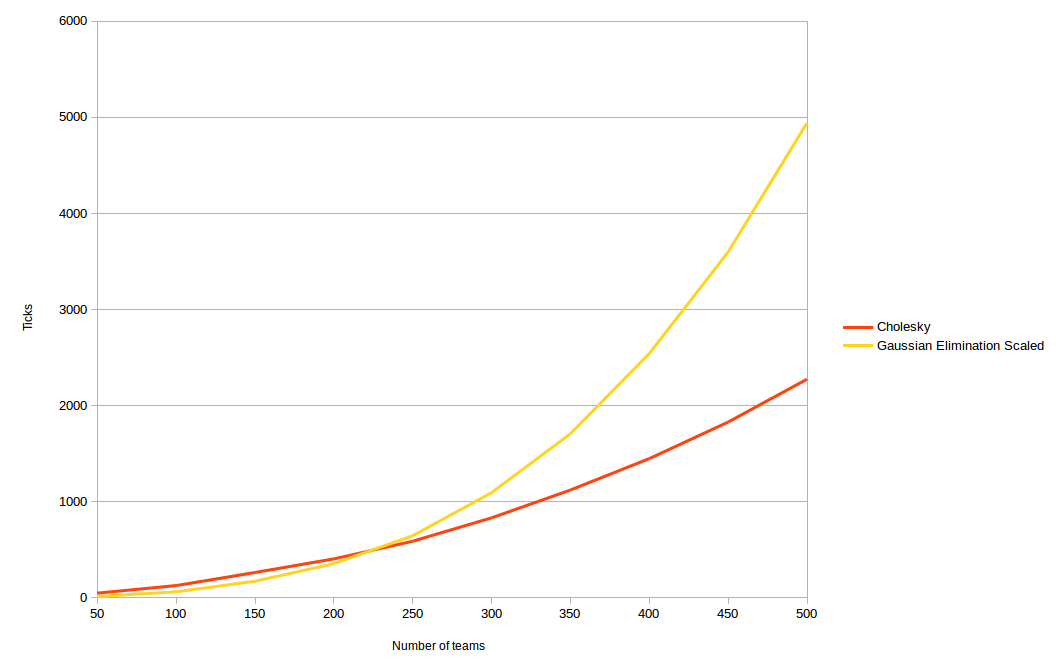
\includegraphics[scale=0.50]{imagenes/cuantitative/bChange/ColleyMatrixCuantitativeBChangeAnalysis.png}
	\caption{Comparaci\'on de complejidad temporal modificando el b en cada iteraci\'on}
	\label{bChange}
  \end{center}
\end{figure}

Este gr\'afico tiene la curva de la Eliminaci\'on Gaussiana escalada para poder visualizarlo en conjunto con la otra.

Puede apreciarse que el m\'etodo de Gauss tiene una curva mucho m\'as pronunciada que la factorizaci\'on y se parecen a las de las complejidaded esperadas. No obstante no podemos discernir si son la misma pero multiplicadas por una constante, de modo que el p\'roximo paso es suavizarlas.

\begin{figure}[h!]
  \begin{center}
	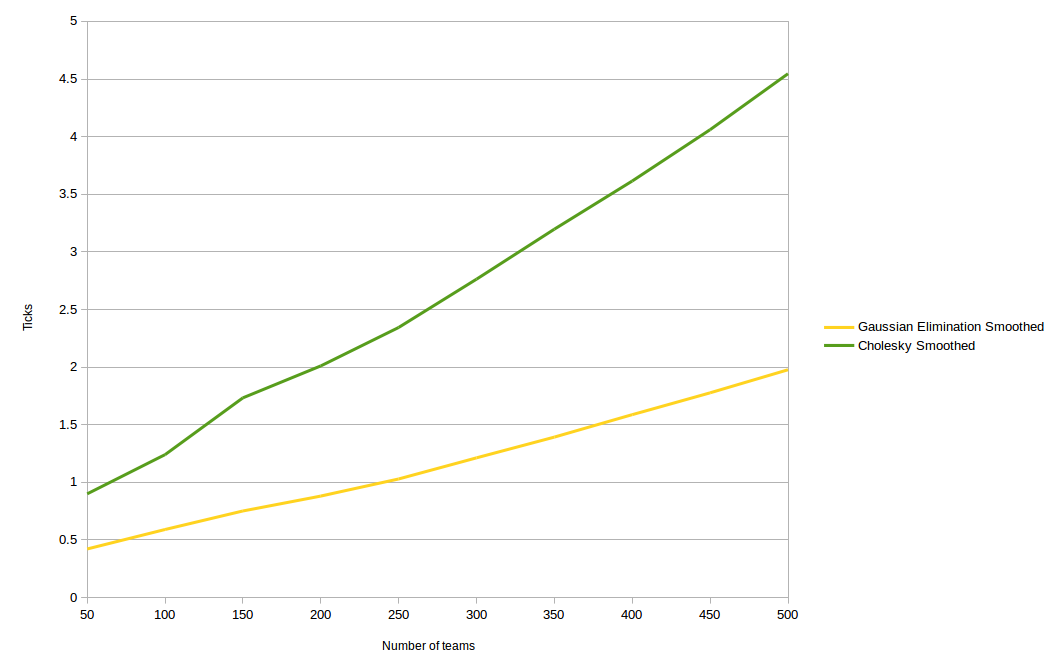
\includegraphics[scale=0.50]{imagenes/cuantitative/bChange/ColleyMatrixCuantitativeBChangeAnalysisSmoothed.png}
	\caption{Comparaci\'on de complejidad temporal modificando el b en cada iteraci\'on suavizado}
	\label{bChangeMoreSmoothed}
  \end{center}
\end{figure}

\newpage

La curva de Gauss fue dividida por el cuadrado del tama\~no de la entrada, mientras que Cholesky fue dividivo por el tama\~no de la entrada. Ambas se ven lineales, de modo que podr\'iamos pensar que la hip\'otesis es correcta. No obstante, vamos a dividir nuevamente a cada curva por el tama\~no de la entrada y ver si la resultante se parece a una funci\'on constante.

\newpage

\begin{figure}[h!]
  \begin{center}
	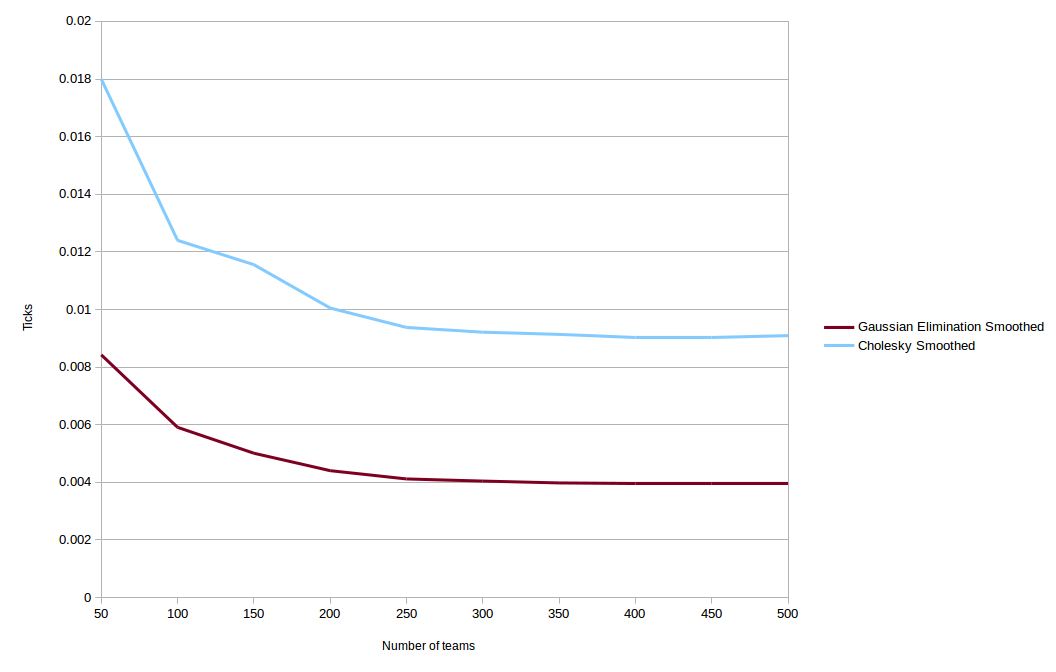
\includegraphics[scale=0.50]{imagenes/cuantitative/bChange/ColleyMatrixCuantitativeBChangeAnalysisConstant.png}
	\caption{Comparaci\'on de complejidad temporal modificando el b en cada iteraci\'on suavizado}
	\label{bChangeSmoothed}
  \end{center}
\end{figure}

Efectivamente, a partir de muestras de tama\~no 250 se aprecia que ambos algoritmos tienden a una constante. Las instancias de n peque\~nos tienen una cantidad de ticks levemente mayor pero, esto es atribuible a motivos de cach\'e del procesador y procesos paralelos.

\subsection{An\'alisis Cualitativo}
\subsubsection{Caracter\'isticas distintivas de los m\'etodos}
Teniendo en una mano el \textit{CMM} y en la otra el \textit{Winning-Percentage}, uno estar\'ia tentado a atinar una respuesta a la pregunta "¿C\'omo se comparan?". En esta secci\'on vamos a presentar resultados a partir de los cu\'ales se puedan observar diferencias o similitudes.

Veamos qu\'e ocurre cuando ponemos a prueba ambos m\'etodos en la NBA con la condicion de que todos los equipos disputaron \textit{aproximadamente} 41 encuentros, que es la mitad de una temporada regular. Los resultados que obtuvimos fueron los siguientes: \\

\textcolor{red}{\textbf{INSERTAR IM\'AGENES CON GR\'AFICOS}} \\

Se puede observar claramente que no hay diferencias substanciales y esto tiene que ver con que observamos un caso \textit{"promedio"}. Una explicaci\'on m\'as matem\'atica yace en lo planteado en \textbf{[1]}, en el estimador de $r_{i}$, obtenido a partir de la \textbf{Regla de sucesi\'on de Laplace [2]}. Ocurre que $r_{i} = \frac{1 + w_{i}}{2 + n_{i}} \approx \frac{w_{i}}{n_{i}} \approx \frac{w_{i}}{k}$ donde este \'ultimo termino es el valor exacto que se obtiene de plantear el \textit{Winning-Percentage} sobre el equipo $i$, para este escenario. Por ende, tiene sentido este parecido.

Pero esto ocurre en un caso real, y la realidad tiende a comportarse en parecido al promedio. Contrastemos esto con casos particulares. \\

\textbf{Hipotesis}: Al ser un simple ``ganados'' / ``totales'', vemos p\'erdida de infomaci\'on sobre el contrincante que puede ocasionar desfasajes importantes.

Para este experimento, lo plantedo fue un conjunto de participantes $\Gamma = \{1,2,...,5\}$, donde se pone al equipo $1$ en la siguiente situaci\'on:

\textcolor{red}{\textbf{INSERTAR IMAGEN experimento_3.in}} \\

El equipo $1$ en 4 ocasiones vence al equipo $2$, 3 al equipo $3$, 2 al equipo $4$ y, finalmente, 1 al contricante $5$ y los resultados fueron: \\

\textcolor{red}{\textbf{INSERTAR IM\'AGENES CON GR\'AFICOS}} \\

Para ambos casos, el algoritmo WP asigna $r_1 = 1$ y $r_i = 0, i = 2, ..., 6$. \footnote{Esto refuerza el hecho de haber usado \textbf{[2]} en el CMM: no s\'olo posiciona a $1$ como ``semi-dios'', sino que el resto de los equipos tiene el mismo rating habiendo el equipo $2$ perdido 10 encuentros y el resto tener el historial limpio.} En cuanto a ratings respecta, el equipo $2$ es efectivamente el \'ultimo y por ende ocurre lo observado. \\

\textbf{Hipotesis}: El m\'etodo CMM previene ``sobre-dimensionar'' a un equipo venciendo reiteradamente a un equipo con bajo ranking, en contra posici\'on al WP. En otras palabras, esto quiere decir que no deber\'ia implicar el mismo aumento de rating vencer a a otro participante con elevado rating que uno con rating pobre. \\

La configuraci\'on del schedule que buscamos para ejemplificar nuestra hipotesis fue uno tal que tenemos $\Gamma = \{1,2,...,4\}$ en el cual los equipos $1$, ..., $3$ juegan entre s\'i y, por ende, podemos armar un rating \textit{parcial} entre ellos. Luego, hacemos jugar al parcialmente ``peor'' jugador, entre los mismos, contra el equipo $4$ de tal forma que ambos algoritmos generan casos distintos. Esta fue la configuraci\'on: \\

\textcolor{red}{\textbf{INSERTAR IMAGEN experimento_3.in}} \\

Y el resultado fue: \\

\textcolor{red}{\textbf{INSERTAR IMAGEN experimento_3.out}} \\

La ``l\'ogica'' indica que ganarle al peor de un grupo no deber\'ia implicar un ascenso importante en los ratings, mucho menos ser mejor o igual que el primero, y en este caso comprobamos que el WP no siempre sigue esa l\'ogica.



\subsubsection{El m\'etodo es justo?}
\textbf{Hip\'otesis:} El algoritmo genera el raiting de cada equipo en base a los raitings de los equipos contra los que jug\'o. Si un equipo no jug\'o contra nadie su rating es 1/2. Cuando el equipo A gana un juego, todos los dem\'as equipos a los que le gan\'o van a tener un mayor rating ya que A ahora gan\'o m\'as partidos y es m\'as valioso. Si un equipo B no jug\'o nunca contra ning\'un equipo que haya jugado con A, el resultado de un nuevo partido de A no debe afectar a B.

Para graficar y analizar la situaci\'on vamos a graficar a los equipos como nodos de un grafo, y cada partido ganado es una arista dirigida con sentido al equipo que perdi\'o.

Adem\'as, vamos a dividir a la hip\'otesis en partes. Primero analizamos que pasa cuando tenemos varios equipos (por ejemplo 5 como en la figura) corriendo la instancia correspondiente obtenemos que los 5 equipos tendr\'an rating igual a 1/2, como quer\'iamos ver.

\newpage

\begin{figure}[h!]
  \begin{center}
	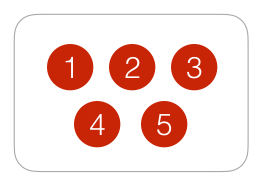
\includegraphics[scale=0.50]{imagenes/cualitative/fairness/fairness1.png}
	\caption{Equipos que no juegan nunca entre s\'i}
%	\label{bChange}
  \end{center}
\end{figure}

Luego tomamos un grafo no conexo como el de la figura siguiente. Usando el CMM vemos que como dice la hip\'otesis, el rating de los equipos 1, 2, 3 y 4 no cambia al variar el resultado de los partidos entre el grafo conexo de 5, 6 y 7.

\begin{figure}[h!]
  \begin{center}
	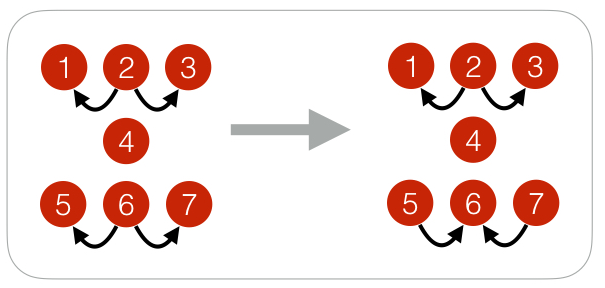
\includegraphics[scale=0.50]{imagenes/cualitative/fairness/fairness2.png}
	\caption{Modificaci\'on de resultado de partidos en subconjunto no conexo}
%	\label{bChange}
  \end{center}
\end{figure}

Ahora que vimos que el resultado de un partido solo puede afectar a los nodos tales que existe un camino entre ellos, veamos el caso de un grafo conexo. Analizamos c\'omo afecta el resultado de un partido donde uno de los jugadores tanto gan\'o como perdi\'o contra otros equipos y queremos ver c\'omo afect\'o al rating de los otros equipos.
Antes de jugar el equipo 4 contra el 2 nos encontramos en una situaci\'on donde 2 tiene rating 1/2 y luego 1 es el que mayor rating tiene ya que le gano a 3 y a 4, luego 3 y 4 tienen mayor rating que 5, 6, 7 y 8.
En el caso de que 4 le gane a 2, podemos observar utilizando el CMM que el equipo 1 aumenta su rating, como enunciamos en la hip\'otesis. Esto se da ya que 4 tiene m\'as partidos ganados y es m\'as valioso ganarle a 4 ahora que antes. Adem\'as el equipo 2 disminuye su rating ya que antes no hab\'ia perdido y ahora s\'i. Pero lo extraño que observamos es que todos los equipos excepto el 2 aumentan su rating, incluso los que est\'an muy poco relacionados, como el equipo 5. Esto se da ya que el rating de cada equipo est\'a en relaci\'on al rating de los equipos contra los que jug\'o. Y al aumentar el rating de 4, aumenta el rating de 1 ya que 1 jug\'o contra 3 y contra 4. Por eso mismo aumenta el de 3, luego 5 y 6, etc.
Para el caso de que 4 pierde contra 2 observamos la misma situaci\'on solo que 2 ahora aumenta su rating y todo el grafo excluyendo al 2 lo disminuye.

Tambi\'en analizando los n\'umeros m\'as en detalle pudimos observar que la jugada entre 2 y 4 afecta en proporci\'on mucho mayor a los ratings de 2 y de 4 que al resto. De hecho cuantas m\'as aristas de distancia m\'as disminuye el impacto en el rating al punto de que el cambio en 5 y 6 es muy poco significativo.

\newpage

\begin{figure}[h!]
  \begin{center}
	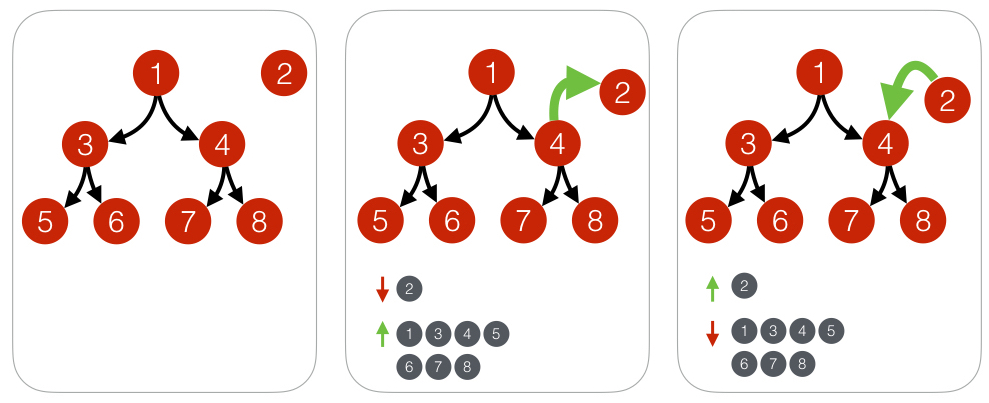
\includegraphics[scale=0.50]{imagenes/cualitative/fairness/fairness3.png}
	\caption{Modificaci\'on de raitings en base al resultado de un partido}
%	\label{bChange}
  \end{center}
\end{figure}

Por \'ultimo analizamos un caso particular donde el resultado de un partido indir\'ectamente puede alterar el ranking de otros equipos que no participaron de ese partido. En el ejemplo de la figura siguiente, el equipo 1 tiene muchos partidos ganados mientras que el 2 no tanto. Sin embargo si el equipo 2 le gana un partido al 1, los equipos 4 y 6 intercambian su posici\'on en el ranking. Esto es un comportamiento muy poco esperado o poco intuitivo ya que por ejemplo podr\'ian darse casos donde un equipo tiene la capacidad de decidir perder para afectar a otro equipo.

\begin{figure}[h!]
  \begin{center}
	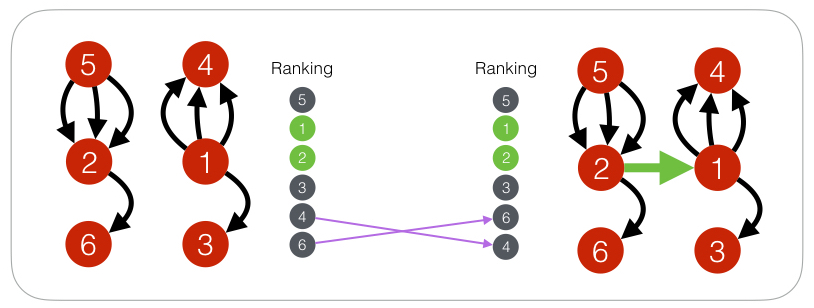
\includegraphics[scale=0.50]{imagenes/cualitative/fairness/fairness4.png}
	\caption{Modificaci\'on de rankings en base al resultado de un partido}
%	\label{bChange}
  \end{center}
\end{figure}

Conclusiones: Aunque creemos que el CMM aporta mucho valor al lograr que ganarle a un equipo que gana mucho aumente m\'as el rating que ganarle a un equipo que gana poco, notamos comportamientos que no son quiz\'as tan intuitivos para establecer los resultados del juego. Algunos ejemplos de esto son los mencionados anteriormente como que no queda tan claro por qu\'e a veces suben los ratings de unos equipos al ganar otros, o el hecho de que el resultado de un partido pueda alterar el ranking de otros que no participaron en ese partido. De todos modos creemos que es una muy buena aproximaci\'on para un manejo m\'as real de los resultados de una competencia.


\subsubsection{Mejor estrategia}
Este apartado surge de la idea de analizar si es posible que un equipo alcance la cima del ranking, si los resultados hubieran sido distintos. Es decir, contamos con un schedule fijo, seleccionamos un equipo participante y tenemos la posibilidad de modificar los partidos perdidos del mismo a ganados. Interesa minimizar la cantidad de modificaciones de este estilo tal que el equipo seleccionado quede en primera posici\'on.

La estrategia que planteamos es la siguiente:

Sea EQUIPO* el equipo que interesa analizar

Calculamos los rankings con la entrada original.

Si ranking(EQUIPO*) es el m\'aximo retornamos la cantidad de iteraciones.

Si no, buscamos el equipo con m\'aximo ranking tal que EQUIPO* tenga alg\'un partido perdido que pueda ser modificado.

Se invierte el resultado y recalculamos los rankings con este cambio.

En caso de que sea imposible modificar un partido (ya se modificaron todos los posibles), retornamos la posicion final.

\textbf{Hip\'otesis:} Los equipos con m\'as derrotas deber\'an modificar m\'as resultados que los que tienen menos. Se espera que la cantidad de partidos ganados por el equipo modificado se aproxime a los que necesit\'o el primero para estar en esa posici\'on. 

Estos fueron los standings finales de la temporada 2014-2015 de la NBA. A la derecha figura la cantidad de partidos que cada equipo deber\'ia ganar en vez de perder para quedar en la primera posici\'on seg\'un nuestro m\'etodo. \\

\begin{tabular}{|c|c|c|c|}
\hline
Posici\'on & Equipo & Record & Ranking\\
\hline
1 & Golden State & 67-15 & 0 \\
\hline
2 & Atlanta & 60-22 & 8 \\
\hline
3 & Houston & 56-26 & 7 \\
\hline
4 & LA Clippers & 56-26 & 8 \\
\hline
5 & Memphis & 55-27 & 10 \\
\hline
6 & San Antonio & 55-27 & 11 \\
\hline
7 & Cleveland & 53-29 & 14 \\
\hline
8 & Portland & 51-31 & 13 \\
\hline
9 & Chicago & 50-32 & 18 \\
\hline
10 & Dallas & 50-32 & 13 \\
\hline
11 & Toronto & 49-33 & 18 \\
\hline
12 & Washington & 46-36 & 21 \\
\hline
13 & New Orleans & 45-37 & 19 \\
\hline
14 & Oklahoma City & 45-37 & 19 \\
\hline
15 & Milwaukee & 41-41 & 26 \\
\hline
16 & Boston & 40-42 & 27 \\
\hline
17 & Phoenix & 39-43 & 25 \\
\hline
18 & Brooklyn & 38-44 & 29 \\
\hline
19 & Indiana & 38-44 & 30 \\
\hline
20 & Utah & 38-44 & 26 \\
\hline
21 & Miami & 37-45 & 29 \\
\hline
22 & Charlotte & 33-49 & 33 \\
\hline
23 & Detroit & 32-50 & 35 \\
\hline
24 & Denver & 30-52 & 35 \\
\hline
25 & Sacramento & 29-53 & 34 \\
\hline
26 & Orlando & 25-57 & 41 \\
\hline
27 & LA Lakers & 21-61 & 44 \\
\hline
28 & Philadelphia & 18-64 & 48 \\
\hline
29 & New_York & 17-65 & 50 \\
\hline
30 & Minnesota & 16-66 & 47 \\
\hline
\end{tabular} \\

Golden State qued\'o en primera posici\'on y por lo tanto requiere 0 partidos para tener el mejor ranking. No es algo sorprendente, pues adem\'as ganaron los Play-Off. Para los dem\'as equipos, la estrategia les pide alcanzar una cantidad de partidos similar a la obtenida por Golden State.

Hay un caso interesante entre Portland, Chicago y Dallas, donde Chicago tiene el mismo record que Dallas, pero necesita 5 partidos m\'as que los otros dos equipos. Esto se debe al schedule de cada uno. Seguramente Chicago jug\'o pocos partidos frente a los equipos por encima de \'el, y probablemente haya ganado algunos. Mientras que Portland y Dallas deben haber jugado m\'as veces contras los mejor rankeados y perdido en varias oportunidades, con lo que una modifici\'on en esos partidos, les significa un salto mayor en la trepada por el ranking.

Probamos tambi\'en qu\'e sucede en el caso en que por ejemplo Golden State, ganara absolutamente todos los partidos. ¿Cu\'antos encuentros deber\'an ganar los dem\'as equipos para tener un ranking mejor?

Los resultados refuerzan, como se present\'o anteriormente, las hip\'otesis planteadas, pidi\'endole a cada equipo que ganara cerca de 80 partidos sobre 82 totales (ganar en vez de perder con Golden State para disminuir su ranking y ganarle a casi todos los dem\'as pues ellos lo hab\'ian hecho).

\newpage
\section{Conclusiones}
\section{Conclusiones}
\newpage
\section{Referencias}
\textbf{[1]} An\'alisis Num\'erico, p\'agina 491 - Burden \& Faires
\newpage
\section{Apendice}
\input{apendice}

%\begin{figure}
%  \begin{center}
%	
\includegraphics[scale=0.66]{imagenes/logouba.jpg}
%	\caption{Descripcion de la figura}
%	\label{nombreparareferenciar}
%  \end{center}
%\end{figure}

%\paragraph{\textbf{Titulo del parrafo} } Bla bla bla bla.
%Esto se muestra en la figura~\ref{nombreparareferenciar}.

%\begin{codesnippet}
%\begin{verbatim}
%
%struct Pepe {
%
%    ...
%
%};
%
%\end{verbatim}
%\end{codesnippet}

\end{document}

